\documentclass[11pt]{ctexart}
\usepackage{graphicx}
\usepackage{amsmath}
\usepackage{booktabs}
\usepackage{cite}
\usepackage{float}
\usepackage{indentfirst}
\usepackage[colorlinks,linkcolor=black]{hyperref}
\usepackage{url}

\setlength{\parindent}{2em}

\usepackage{minted}

\title{OSH详细设计报告\\[2ex]实时文本协作系统}
\author{徐直前 PB16001828\\吴永基 PB16001676\\黄子昂 PB16001840\\金朔苇 PB16001696\\}
\date{\today}
\begin{document}

\maketitle
\tableofcontents

\section{项目概述}
在本项目中,我们参考了有关CRDT的论文,用JavaScript实现了一个基于状态的CRDT,并在此CRDT基础上用JavaScript和Node.js编写前后端,最终实现了一个基于网页端,轻量,能以类似C等语言中
花括号的方式实现块级的权限控制,并且能够对Markdown语法支持以及实现实时预览,也具有一定的鲁棒性。其主要特征如下:
\begin{itemize}
    \item 基于CRDT实现,具有很好的可伸缩性;
    \item 采用纯JavaScript编写,为网页端应用;
    \item 使用Node.js作为后端,利用npm包管理器可以很方便地完成部署;
    \item 支持Markdown,并支持实时预览;
    \item 能实现精确到块级的权限控制,管理员可以指定某块内容只能由某个用户编辑,同时也可以指定一个公共的编辑区域;
    \item 具备高度可再开发性,基于本项目可以实现更高级的实时文本协作应用。
\end{itemize}

目前权限管理采用免登陆的方式,第一个登陆网页的人即为管理员(admin),此后登陆的人都为普通用户(guest)。仅有管理员拥有全部权限,
可以控制普通用户的编辑权限。而普通用户不能进行权限的编辑。
管理员权限也会动态转移。当当前管理员离线时,管理员权限会即可转移到第一个guest上。
这种免登陆的权限控制实施方案极适用于一个团队在同一个局域网内进行实时协作。当然,也可以维护一个相应的用户数据库,实现用户名密码登陆的用户管理方式,
此部分内容在本项目基础上很容易扩展,而且与实时文本协作的核心技术难题无关,故没有实现该种方式。

我们将本项目部署在了一台腾讯云服务器上,并且也在结题汇报时进行了现场互动演示,实现了很好的效果。
\begin{figure}[ht]
    \begin{center}
    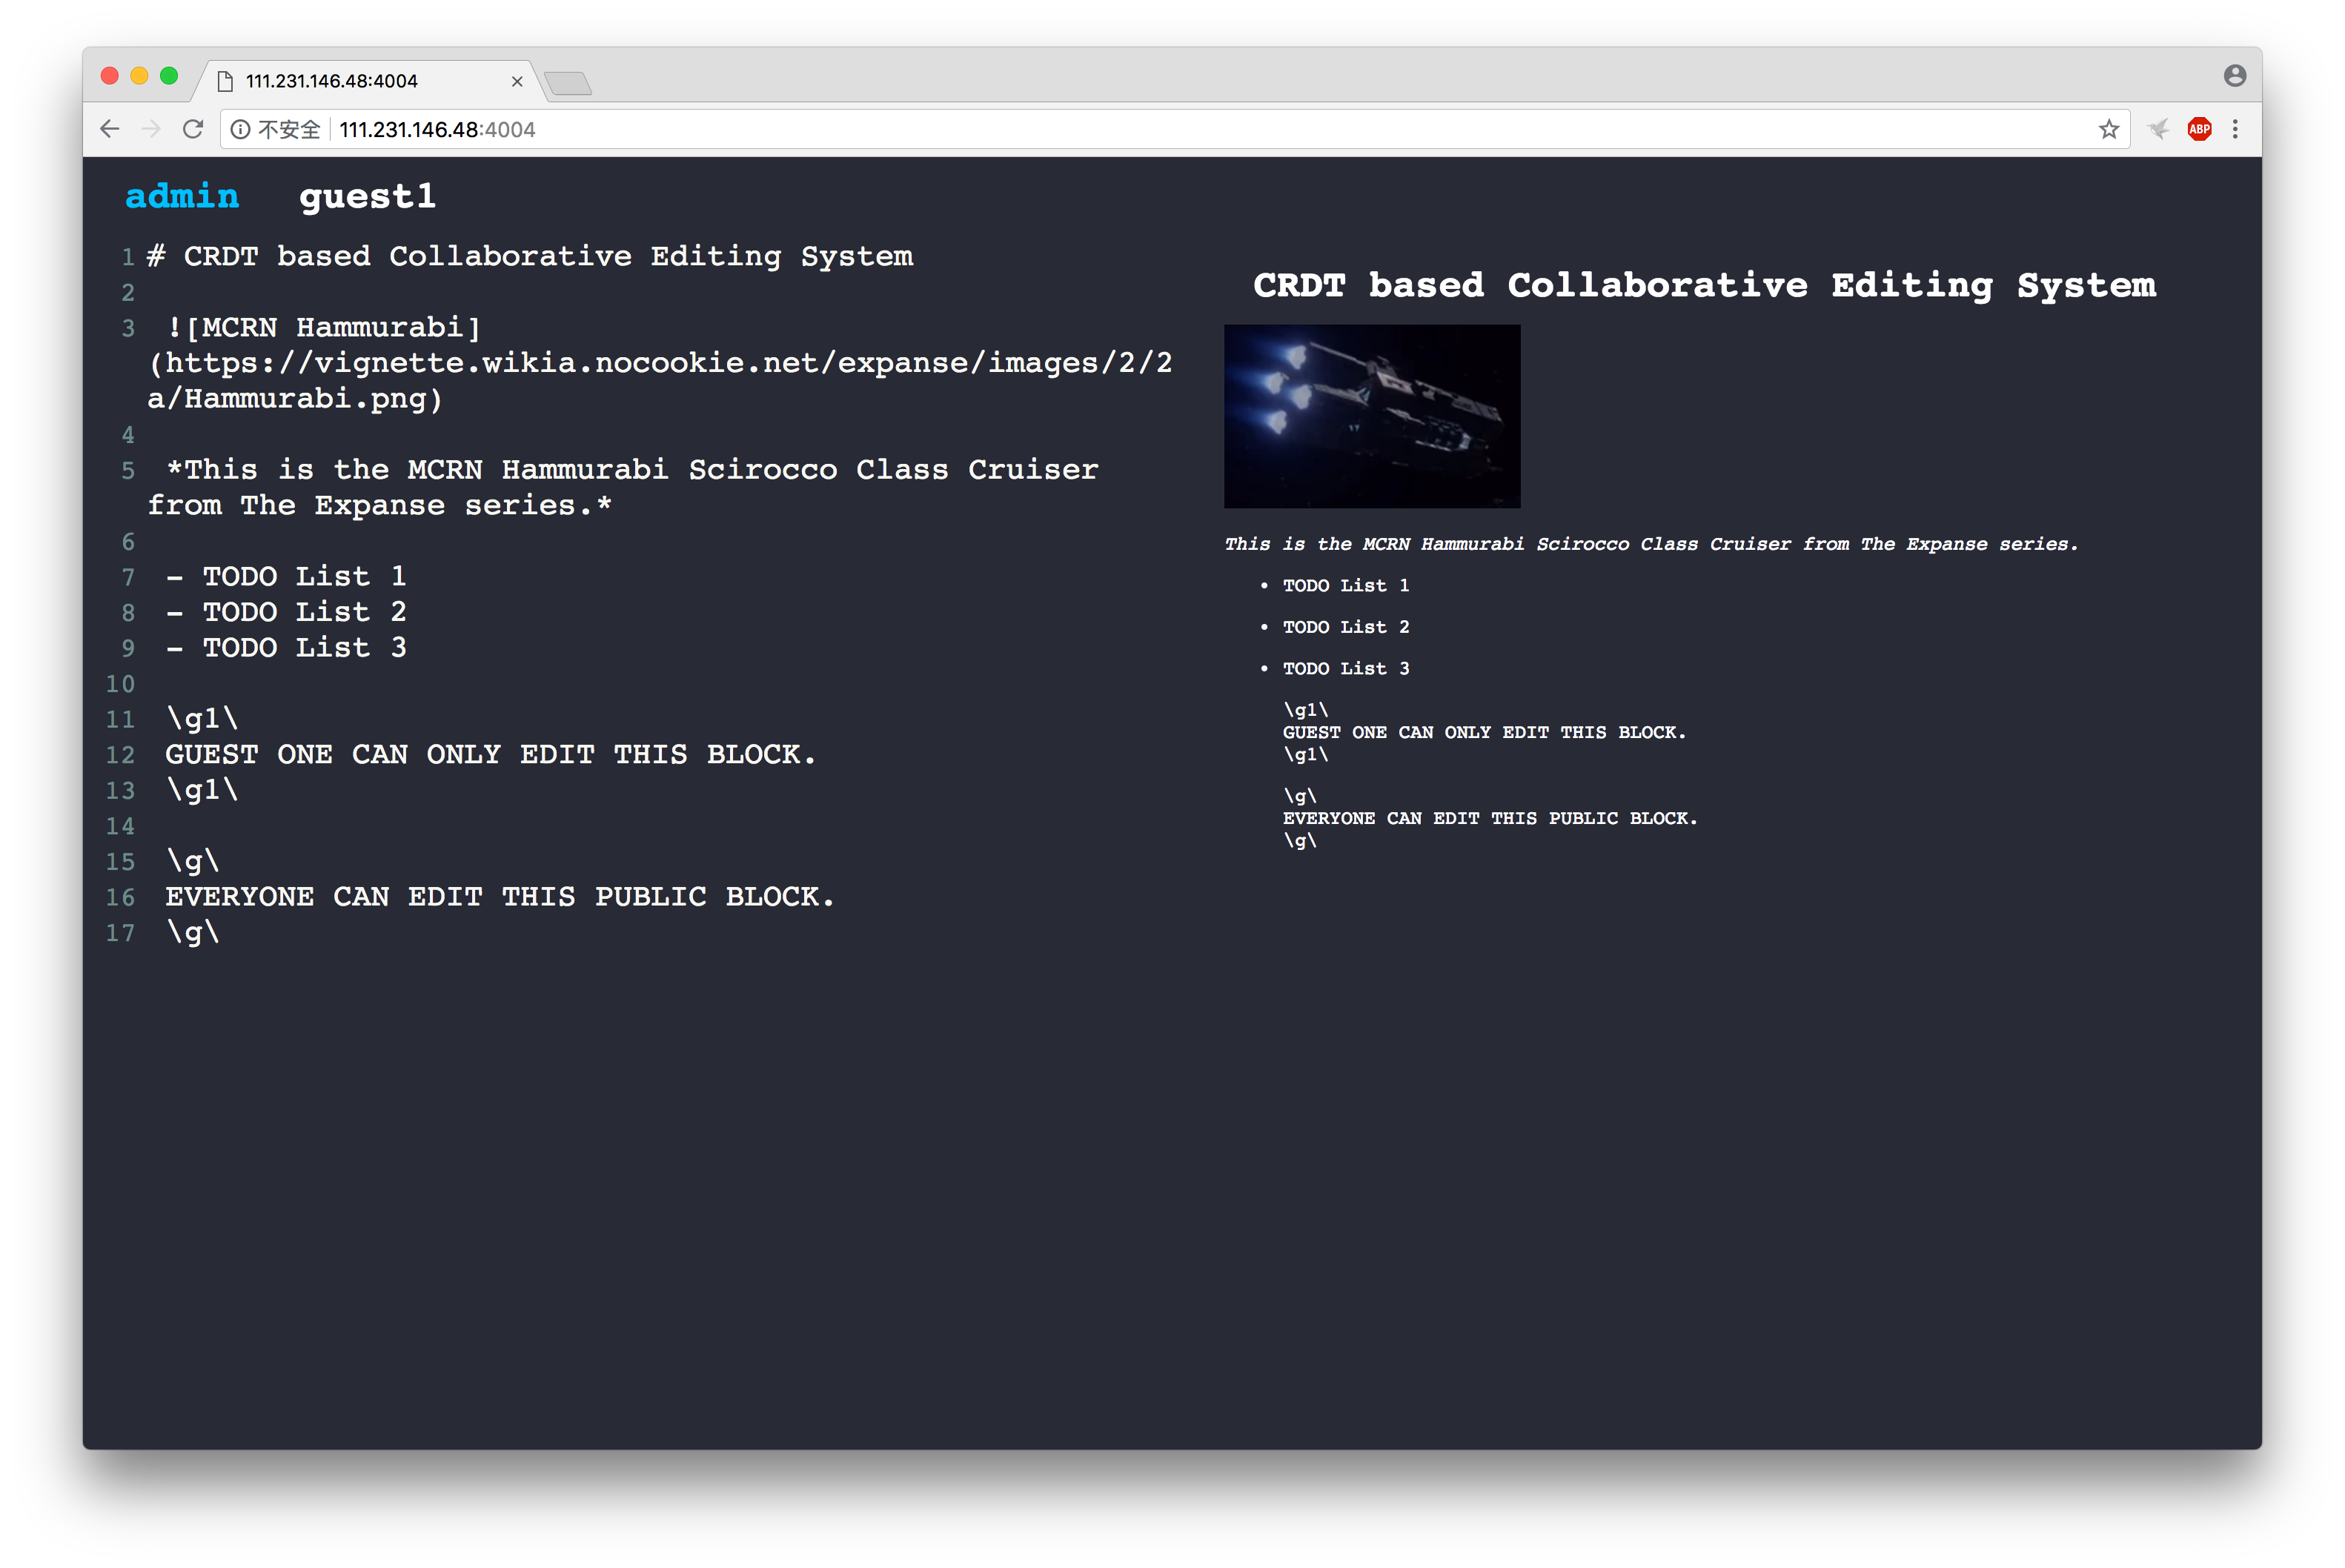
\includegraphics[width=\textwidth]{figures/demo.png}
    \caption{最终实现效果}
    \end{center}
\end{figure}
\section{背景知识}
本部分内容将介绍与此项目相关的背景知识,其部分内容在调研报告和可行性报告中也有所介绍,在此也对其中的关键内容进行一下回顾。
\subsection{实时文本协作的技术难点}
实时文本协作从用户层面来说看似十分简单,然而其面对的技术难题却是相当巨大的。业界在此问题上也进行了几十年的研究,最终也才在近些年来诞生了像Google Docs这样较为
完善的实时文本协作系统。其主要的难点在于解决不同用户的数据副本之间的同步问题。  

通常在这种高交互性的网络应用中,为了隐藏网络延时对用户体验带来的影响,我们要在每个客户端上
保存一个本地的用户副本。每个用户的操作都直接在本地数据副本上执行,这样本地的操作就不会受到网络延时的影响,用户能获得很好的本地响应性。
然而,这样的方式也会带来问题。需要设计一种机制维持各个用户的数据副本之间的一致性。如果用户的副本出现了不一致的情况,
那么显然会导致灾难性的后果。

我们用一个具体例子来说明其中的技术难题。假设现有Alice和Bob两人同时进行文档的编辑。
初始状态下Alice和Bob各自的副本都是相同的,内容如下:
\begin{center}
\textit{We wanted cars, instead we got characters.}
\end{center}

此时Alice想在 \textit{got} 后面插入 \textit{140} ,同时Bob又想在 \textit{wanted} 后面插入 \textit{flying}。
如果网络没有任何延时,所有的操作都能被瞬间应用,而Alice和Bob之间的操作在物理上也必然会有个先后关系,两者的操作会按照时间的先后关系而被执行,
这里我们就不会遇到任何问题了。
但是,由于网络有延时,那么问题就来了。Alice和Bob两个人各自都先执行自己的本地编辑操作,Alice先会进行一个 \textit{insert(140, col=30)} 的操作,在第30个位置插入
字符串 \textit{140} ,同样Bob先会执行的操作是 \textit{insert(flying, col=9)} 。此后,Alice和Bob分别将自己进行的操作广播给对方
Alice受到Bob的操作后然后执行 \textit{insert(flying, col=9)} ,Bob收到Alice的操作后执行 \textit{insert(140, col=30)} 。

此时,对Alice来说一切正常,她得到的状态是:
\begin{center}
    \textit{We wanted flying cars, instead we got 140 characters.}\footnote{Peter Thiel的名句,讽刺了人类似乎点错了科技树,近些年来除了互联网领域有飞跃性的进展,
    我们的科技缺少从0到1的突破。}
\end{center}

但Bob就糟糕了,此时Alice实际想要插入的位置就不是第30个位置了。Bob的状态变成了:
\begin{center}
    \textit{We wanted flying cars, instead 140 we got characters.}
\end{center}

显然,Alice和Bob得到了不一致的结果,这显然是文本协作中不能容忍的。为此,我们的核心问题就是通过一种什么样的机制来保证每个用户都能得到相同的数据副本?
\subsection{CRDT}
为了解决上述问题,业界也展开了数十年的研究,很多种方案例如AST(Address Space Transformation)、OT(Operational Transformation)、
WOOT(WithOut Operational Transformation)、CRDT(Conflict-free Replicated Data Type)被相继提出。
目前大多数主流文本协作应用例如Google Docs、石墨文档用的均是OT技术。OT的核心思想非常简单,当远程的操作到达本地站点后,其操作的上下文
可能和相应的客户端发出该操作时不同了,为了正确的执行该操作,我们要在执行远程操作之前对其转换,使得在当前的上下文下执行操作仍然不改变原始操作效果。
由于需要谨慎考虑所有可能出现的情况,OT不具备较好的可伸缩性,同时实现起来也非常复杂。CRDT则是近些年来新提出的一种技术,也正在逐渐被更加深入的研究
和在产品中应用。

CRDT有很多种不同的具体类型和实现,但大体上可以分为两类:基于状态的CRDT和基于操作的CRDT。基于状态的CRDT在更新时会将副本的
整个状态广播给其他副本。当一个副本收到了其他副本的状态时,会根据merge函数的机制和本地的状态进行merge。而基于操作的
CRDT则在每次更新时不广播整个副本的状态,而仅仅广播更新的操作,这样避免了整个状态过大不便于传输的问题。
\begin{figure}[ht]
    \begin{center}
    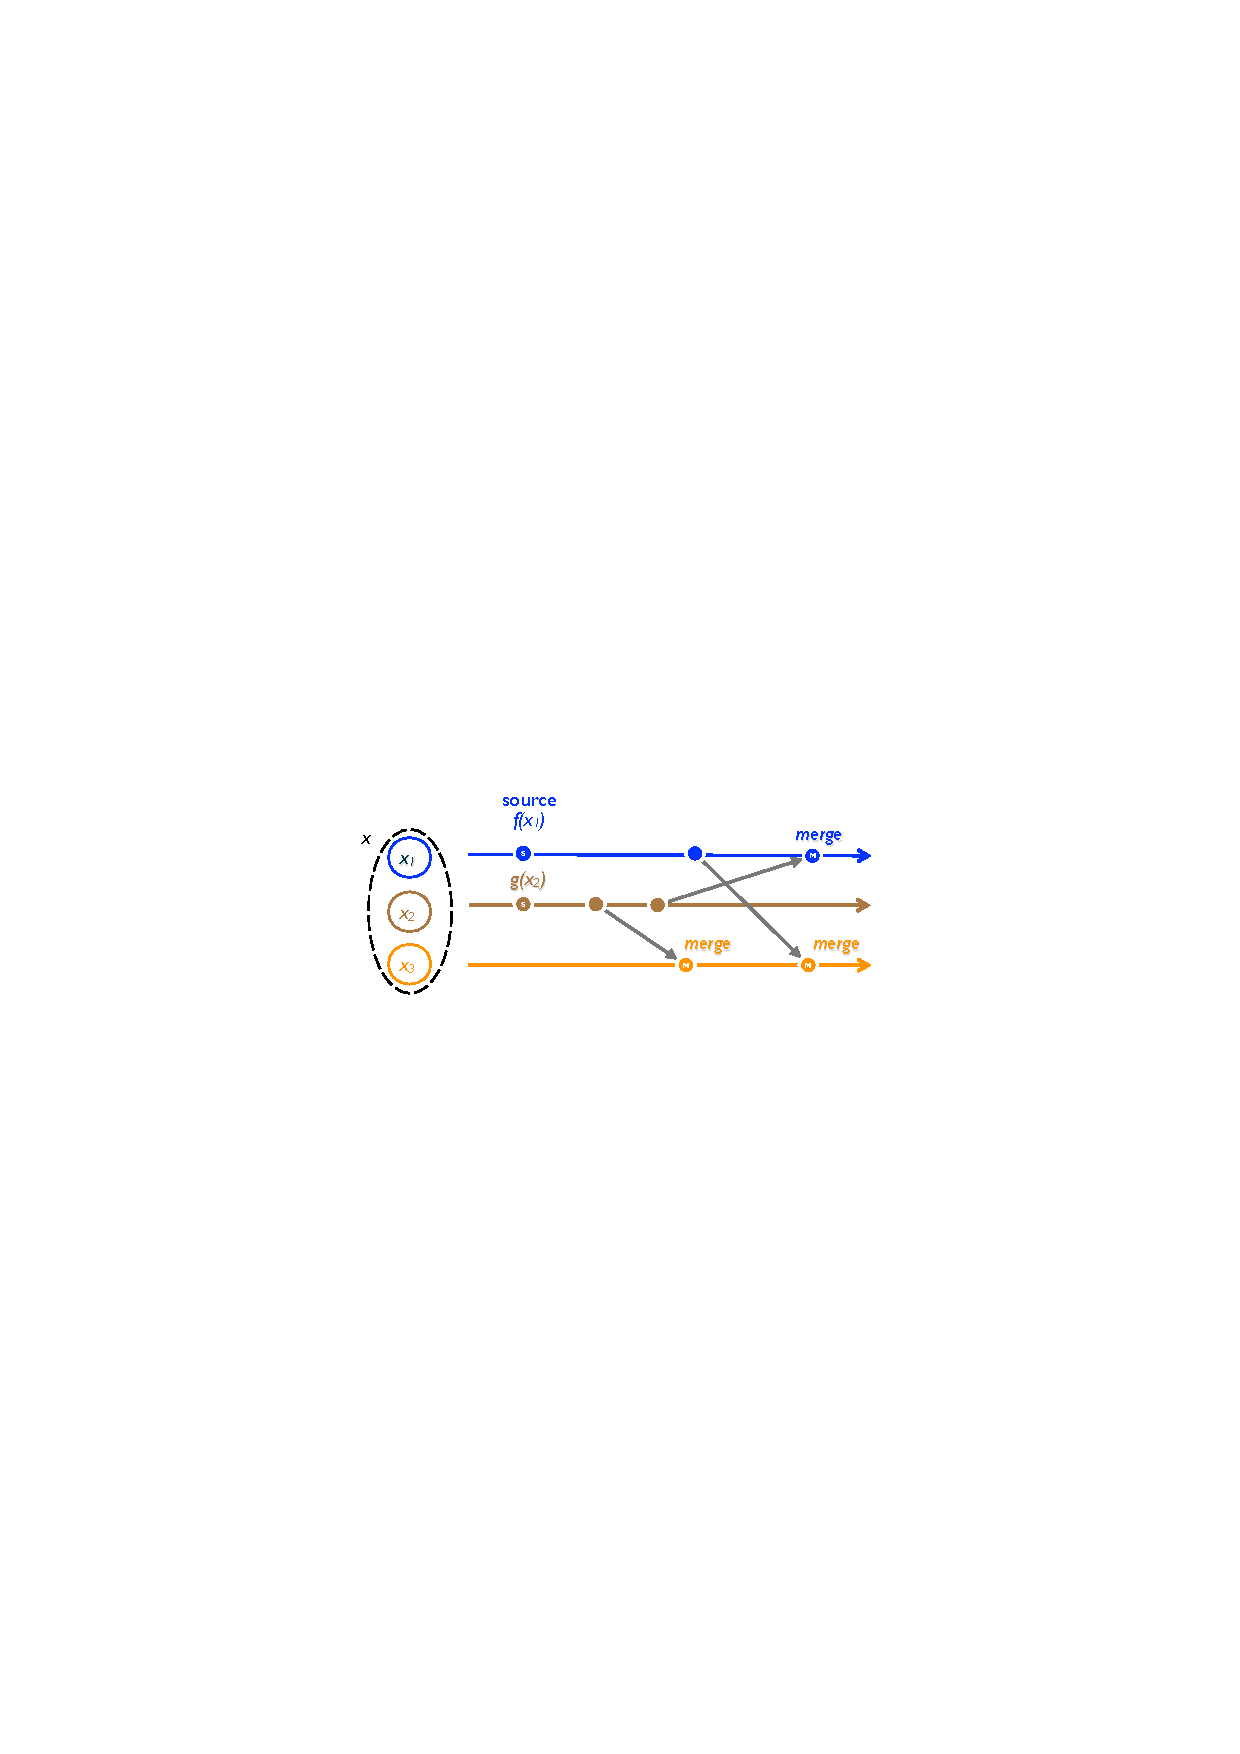
\includegraphics[width=\textwidth]{figures/state_crdt.pdf}
    \caption{基于状态的CRDT}
    \end{center}
\end{figure}

在该项目中我们采用了一种基于状态的CRDT实现文本协作,通过给文本中的每一个字符一个独一无二的标识符,我们将一个文本文档转换成了
一个有序的标识符序列。通过这个标识符序列,我们可以很轻松地维护各个副本之间一致性。CRDT这种数据类型能够使得并发操作之间相互commute。如果操作
是以先行发生(happen-before)的顺序产生,那么CRDT的副本之间不需要复杂的并发控制就能自动收敛达成一致。

在文本实时协作中,我们给每一个原子(也就是每一个字符)赋予一个独一无二的位置标识符(PosID),满足一下三条原则
\begin{enumerate}
	\item 每一个在缓冲区中的原子都有一个ID
	\item 任意两个不同的原子都有两个不同的ID
	\item 一个给定原子的ID在整个文档剩余的生命周期中保持不变
	\item ID之间有一个全序关系,和原子在缓冲区中的顺序一致
	\item ID取值空间是密集的,即:$\forall P, F : P < F \Rightarrow \exists N: P < N < F$
\end{enumerate}
我们定义一个抽象的原子数据缓冲区的状态T是一个由 (\textit{atom,PosID}) 二元组构成的集合,状态T的内容就是由T中所有原子按照\textit{PosID}排列构成的序列。 

每一个用户都会维持这个CRDT的一个副本,并且进行本地编辑
\begin{itemize}
	\item \textit{insert}($\mathit{PosID_{n}}$, newatom)
	\item \textit{delete}($\mathit{PosID_{n}}$)
\end{itemize}
这样,两个指向不同的PosID的操作是相互独立的。因为他们对于CRDT的作用效果是与他们的执行顺序无关的。那么现在只需要考虑并发的指向相同的PosID的两个操作。
一个插入操作必定发生在一个删除操作之前签,所以他们不可能是并发的。最后,删除操作是幂等的(idempotent),因为删除掉了一个给定PosID的字符再次删除这个PosID的字符是无效的。
因此,我们这样构建的一个缓冲区就构成了一个简单的CRDT,实现了文本实时协作功能。

但是,在这里还有两个问题需要考虑。
\begin{itemize}
	\item 两个客户端在同一时间生成了同样的PosID(当他们并行地在同一个位置插入字符)
	\item 一个客户端生成了一个已经被使用过的PosID(删除一个字符之后重新插入他们)
\end{itemize}

第二个问题很好解决,每个客户端自己只要维持一个记录,保证不会生成自己已经使用过的PosID即可。第一个问题同样可以用一个很简单的方法解决,我们只要将每一个PosID变成一个二元组即可,把PosID这个标识数字和产生该ID的客户端编号放在一起即可。这样就保证了两个客户端不会产生同样的PosID。
\nocite{*}
\bibliographystyle{plain}
\bibliography{ref}
\end{document}